\documentclass[a4paper, 11pt]{report}
\usepackage[utf8]{inputenc}   % Pour lire les fichiers UTF-8
\usepackage[T1]{fontenc}      % Pour une meilleure gestion des caractères accentués
\usepackage{textcomp}         % Pour quelques symboles supplémentaires
\usepackage{lmodern}          % Police compatible avec T1
\usepackage[english,french]{babel} 
\usepackage{graphicx} % Pour les images
\def\@captype{figure}
\usepackage{float}
\usepackage{multicol} % Pour faire des multi colonnes
\usepackage[export]{adjustbox} % Pour la clé 'valign'  (aligner verticalement)
\usepackage[colorlinks=true,linkcolor=black]{hyperref} % Pour qu'il y est des liens sur la table des matières
\usepackage{caption} % Utiliser plus de fonction sur caption (caption* pour ne pas afficher FIGURE-1)
\usepackage{lipsum} % Pour générer du texte pour voir comment ca rend
\usepackage{ragged2e} % Pour justifier le texte
\usepackage{ulem}
\usepackage[margin=3.2cm]{geometry}
\usepackage{forest}
\usepackage{listings}
\usepackage{xcolor}
\usepackage[section]{placeins}
\usepackage{amsmath}
\usepackage{amssymb}
\usepackage{fancybox}
\usepackage{fancyhdr}
\usepackage[none]{hyphenat}
\emergencystretch=3em
\usepackage{graphicx}
\usepackage{adjustbox}
\usepackage{float}


\usepackage{csquotes}

% Configuration des en-têtes et pieds de page
\pagestyle{fancy}
\fancyhf{}
\fancyhead[C]{Rapport de Projet}
\fancyfoot[L]{2025}
\fancyfoot[C]{COUTANT, LITAMPHA, PETER}
\fancyfoot[R]{\thepage}
\renewcommand{\headrulewidth}{0.4pt}
\renewcommand{\footrulewidth}{0.4pt}
\setlength{\headheight}{13.59999pt}

\fancypagestyle{plain}{
  \fancyhf{}
  \fancyhead[C]{Rapport de Projet}
  \fancyfoot[L]{L3 Informatique}
  \fancyfoot[C]{COUTANT, LITAMPHA, PETER}
  \fancyfoot[R]{\thepage}
  \renewcommand{\headrulewidth}{0.4pt}
  \renewcommand{\footrulewidth}{0.4pt}
}

\begin{document}

% Page de titre
\begin{titlepage}
    \centering
    \vspace{3cm}
    \includegraphics[width=0.4\textwidth]{images/logo_univ.jpg}\hfill
    \includegraphics[width=0.5\textwidth]{images/logo_ufrst.png}\\
    \vspace{1.5cm}
    {\huge \textbf{Université Marie \& Louis Pasteur\\ UFR Sciences et Techniques}\par}
    \vspace{0.5cm}
    \shadowbox{\parbox{0.9\linewidth}{\centering \huge \textbf{Projet L3 : Pacman en réseau}}}\\
    \vspace{1cm}
    {\Large \textbf{Rapport de Projet} \\ Licence CMI Informatique - 3ème année \\ 2025-2026\par}
    \vspace{0.5cm}
    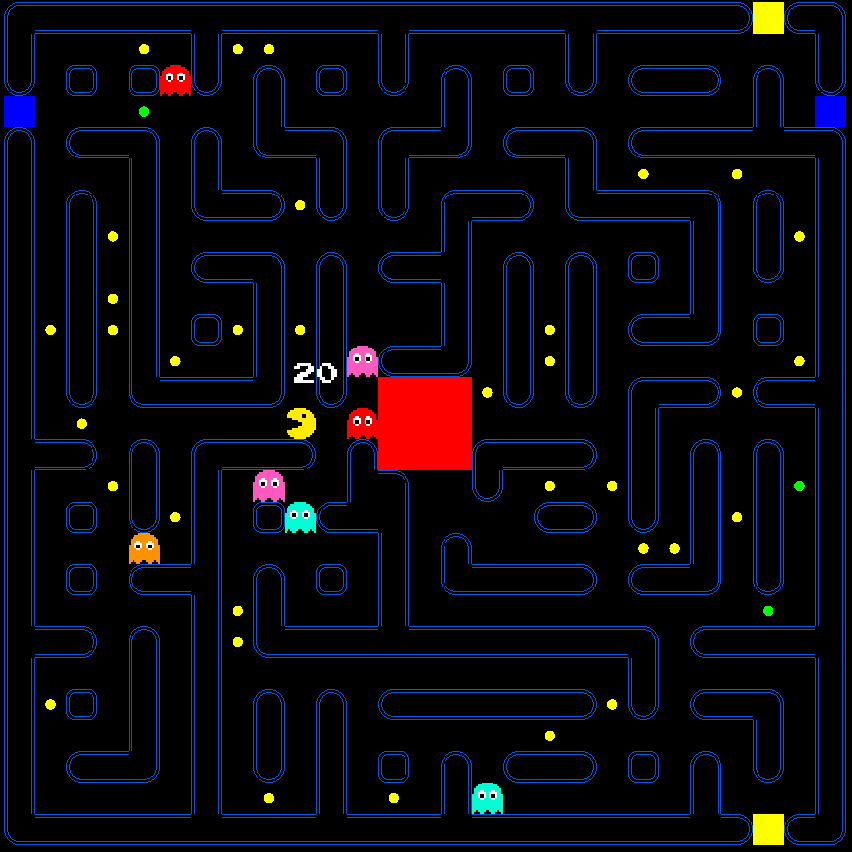
\includegraphics[width=0.7\textwidth]{images/entete.png}\\
    \vspace{0.5cm}
    {\LARGE \textbf{Thomas COUTANT}\\ \textbf{Benoît LITAMPHA}\\ \textbf{Auriane PETER}\par}
    \vspace{1cm}
    {\large \textbf{Encadrant : Julien BERNARD} }\\
\end{titlepage}

\chapter{Introduction}

Le projet de Licence 3 Informatique visait la conception et le développement d’un jeu multijoueur en réseau inspiré de Pac-Man. 
Au-delà du jeu, il mobilisait des compétences clés : architecture client-serveur, synchronisation réseau, génération procédurale, intelligence artificielle et interface graphique.

Le principal défi résidait dans la création d’une architecture autoritaire capable de gérer plusieurs connexions simultanées tout en garantissant la cohérence du jeu. 
Un modèle centralisé côté serveur permet d’assurer l’équité, de limiter les incohérences et de simplifier la validation des actions.

Le projet comportait deux phases : un prototype minimal (mi-octobre à décembre) et trois sprints intensifs d’une semaine chacun en janvier pour produire une version fonctionnelle et stable.

\chapter{Organisation et approche Agile}

\section{Organisation et rôles}

L’équipe se composait de trois étudiants : 

\begin{itemize}
    \item \textbf{Thomas} : développement serveur et chef de sprint,
    \item \textbf{Auriane} : développement client,
    \item \textbf{Benoît} : client et serveur, communication réseau.
\end{itemize}

Les décisions techniques étaient collaboratives, combinant spécialisation et vision d’ensemble.

\section{Communication et outils}

La coordination reposait sur Discord pour les échanges quotidiens et GitHub pour le versionnement et l’historique du code. 
Cette organisation a permis un travail parallèle efficace et une intégration continue des modules.

\section{Phases du projet et fonctionnement des sprints}

\subsection{Prototypage (octobre-décembre)}

Développement d’un prototype minimal pour tester la connexion client-serveur et la synchronisation de base.

\subsection{Sprints intensifs (janvier)}

Trois sprints d’une semaine, chacun concluant sur une version partielle mais fonctionnelle :

\begin{enumerate}
    \item Définition des objectifs,
    \item Développement parallèle,
    \item Communication continue,
    \item Point hebdomadaire avec le tuteur,
    \item Stabilisation et validation.
\end{enumerate}

\chapter{Sprint 1 : Architecture serveur complète}

\section{Objectifs}

Transformer le prototype en une architecture client-serveur complète : gestion de connexions multiples, lobby, rooms, boucle de jeu et génération procédurale.

\section{Refonte du prototype}

La modularisation du serveur a permis de séparer :

\begin{itemize}
    \item gestion des connexions,
    \item lobby,
    \item rooms,
    \item boucle de jeu,
    \item génération du plateau.
\end{itemize}

Chaque room était indépendante pour éviter les interférences entre parties.

\section{Difficultés et résultats}

La principale difficulté fut la transition vers un système multi-room sans régressions. 
Le sprint a abouti à une architecture serveur stable, un lobby fonctionnel et une génération procédurale opérationnelle.

\chapter{Sprint 2 : Développement client et bots}

\section{Objectifs}

Créer un client complet et intégrer les bots IA pour rendre le jeu jouable.

\section{Client et gestionnaire de scènes}

Séparation claire entre :

\begin{itemize}
    \item réseau,
    \item logique locale,
    \item interface graphique.
\end{itemize}

Le gestionnaire de scènes a structuré les menus, lobby et parties, améliorant la maintenabilité.

\section{Synchronisation et bots}

Le serveur reste la source de vérité. 
Les bots, gérés côté serveur, suivent une logique autonome et de poursuite.

\section{Résultats}

Client fonctionnel, synchronisation stable, bots intégrés, expérience de jeu complète.

\chapter{Sprint 3 : Stabilisation et finition}

\section{Objectifs}

Stabiliser le système, corriger bugs, améliorer l’interface graphique et l’expérience utilisateur.

\section{Travail côté serveur et client}

\begin{itemize}
    \item Corrections des transitions d’état,
    \item Optimisation du gestionnaire de scènes,
    \item Simplification des messages réseau,
    \item Harmonisation visuelle du client.
\end{itemize}

\section{Résultats}

Système stable, lobby et rooms fonctionnels, boucle de jeu robuste et interface graphique finalisée.

\chapter{Analyse critique}

\section{Bénéfices de l’Agile}

\begin{itemize}
    \item Validation progressive de l’architecture,
    \item Adaptation rapide aux difficultés techniques,
    \item Communication continue et résolution rapide des problèmes.
\end{itemize}

\section{Limites}

\begin{itemize}
    \item Absence d’outil formel de gestion des tâches,
    \item Sous-estimation de certaines tâches,
    \item Coordination partiellement informelle.
\end{itemize}

\section{Enseignements}

Prototype précoce, architecture modulaire, séparation logique/graphique, sprints courts pour la réactivité.

\chapter{Bilan et retour d’expérience}

\section{Bilan technique}

Compétences mobilisées :

\begin{itemize}
    \item Architecture client-serveur autoritaire,
    \item Gestion des états et synchronisation réseau,
    \item Lobby, rooms, boucle de jeu,
    \item Interface graphique modulable,
    \item Bots IA intégrés.
\end{itemize}

\section{Compétences et méthodologie}

\begin{itemize}
    \item Montée en complexité progressive,
    \item Validation régulière des choix,
    \item Adaptation rapide et communication continue.
\end{itemize}

\section{Axes d’amélioration}

\begin{itemize}
    \item Outil formel de gestion des tâches,
    \item Critères de validation de sprint plus précis,
    \item Formalisation du protocole réseau,
    \item Tests automatisés.
\end{itemize}

\section{Perspective globale}

L’expérience confirme la pertinence d’une architecture solide, d’une organisation méthodique et d’une capacité d’adaptation pour réussir un projet logiciel complexe.

\chapter{Conclusion}

Le projet a permis de transformer un prototype en un système complet et stable, en combinant compétences techniques et organisation Agile. 
L’architecture serveur modulaire, la séparation logique/graphique, la boucle de jeu centralisée et la communication continue ont été déterminantes pour la réussite. 
Cette expérience constitue une base solide pour des projets futurs impliquant architectures distribuées et contraintes techniques fortes.

\end{document}